\chapter{Tecnologie utilizzate}
In questo capitolo verranno descritte le attività preliminari per la realizzazione di questo progetto, le tecnologie utilizzate
unitamente alle motivazioni legate all'uso di questi sistemi rispetto ad altri.

% - nel capitolo sulle tecnologie parlare di python, django, docker? -

\section{Python, Django}
Python è un linguaggio di programmazione ad alto livello, orientato agli oggetti, adatto, tra gli altri usi, a sviluppare applicazioni 
distribuite, scripting, computazione numerica e system testing; ideato e rilasciato pubblicamente per la prima volta nel 1991 dal suo 
creatore Guido van Rossum, programmatore olandese.

Python supporta diversi paradigmi di programmazione, come quello object-oriented (con supporto all'ereditarietà multipla), quello 
imperativo e quello funzionale, ed offre una tipizzazione dinamica forte. È fornito di una libreria built-in estremamente ricca, che 
unitamente alla gestione automatica della memoria e a robusti costrutti per la gestione delle eccezioni fa di Python uno dei linguaggi 
più ricchi e comodi da usare.

Inoltre è anche semplice da usare e imparare. Python, nelle intenzioni di Guido van Rossum, è nato per essere un linguaggio 
immediatamente intuibile. La sua sintassi è pulita e snella così come i suoi costrutti, decisamente chiari e non ambigui. I blocchi 
logici vengono costruiti semplicemente allineando le righe allo stesso modo, incrementando la leggibilità e l'uniformità del codice 
anche se vi lavorano diversi autori.

Un aspetto inusuale del Python è il metodo che usa per delimitare i blocchi di programma, che lo rende unico fra i linguaggi più diffusi.

\lstset{style=python_code_style}
\begin{lstlisting}[language=Python, caption={Esempio di programma in Python}]
def test(got, expected):
	if got == expected:
		prefix = ' OK '
	else:
		prefix = ' X '
	print ('%s got: %s expected: %s' % (prefix, repr(got), repr(expected)))

def main():
	print ('verbing')
	test(verbing('hail'), 'hailing')
	test(verbing('swiming'), 'swimingly')
	test(verbing('do'), 'do')

if __name__ == '__main__':
	main()
\end{lstlisting}

Nei linguaggi derivati dall'ALGOL come Pascal, C e Perl, i blocchi di codice sono indicati con le parentesi oppure con parole chiave 
(il C ed il Perl usano { }; il Pascal usa begin ed end). In questi linguaggi è solo una convenzione degli sviluppatori il fatto di 
indentare il codice interno ad un blocco, per metterlo in evidenza rispetto al codice circostante. Invece Python deriva il suo sistema 
di indentazione dal meno noto linguaggio di programmazione Occam: invece di usare parentesi o parole chiave, usa l'indentazione stessa 
per indicare i blocchi nidificati in congiunzione col carattere "due punti" (:). Si può usare sia una tabulazione, sia un numero
arbitrario di spazi, ma lo standard Python è di 4 spazi. \cite{python-documentation}


Python è un linguaggio pseudocompilato: un interprete si occupa di analizzare il codice sorgente (semplici file testuali con 
estensione .py) e, se sintatticamente corretto, di eseguirlo e non esiste una fase di compilazione separata (come 
avviene in C, per esempio) che generi un file eseguibile partendo dal sorgente.


Django is a high-level Python web framework that enables rapid development of secure and maintainable websites. Built by experienced 
developers, Django takes care of much of the hassle of web development, so you can focus on writing your app without needing to 
reinvent the wheel. It is free and open source, has a thriving and active community, great documentation, and many options for free 
and paid-for support. 

Django helps you write software that is:

Complete
	Django follows the "Batteries included" philosophy and provides almost everything developers might want to do "out of the box". 
	Because everything you need is part of the one "product", it all works seamlessly together, follows consistent design principles, 
	and has extensive and up-to-date documentation.
Versatile
	Django can be (and has been) used to build almost any type of website — from content management systems and wikis, through to 
	social networks and news sites. It can work with any client-side framework, and can deliver content in almost any format 
	(including HTML, RSS feeds, JSON, XML, etc). The site you are currently reading is based on Django!

	Internally, while it provides choices for almost any functionality you might want (e.g. several popular databases, templating 
	engines, etc.), it can also be extended to use other components if needed.
Secure
	Django helps developers avoid many common security mistakes by providing a framework that has been engineered to "do the right 
	things" to protect the website automatically. For example, Django provides a secure way to manage user accounts and passwords, 
	avoiding common mistakes like putting session information in cookies where it is vulnerable (instead cookies just contain a key, 
	and the actual data is stored in the database) or directly storing passwords rather than a password hash.
	Scalable
	Django uses a component-based “shared-nothing” architecture (each part of the architecture is independent of the others, 
	and can hence be replaced or changed if needed). Having a clear separation between the different parts means that it can 
	scale for increased traffic by adding hardware at any level: caching servers, database servers, or application servers. Some 
	of the busiest sites have successfully scaled Django to meet their demands (e.g. Instagram and Disqus, to name just two).
Maintainable
	Django code is written using design principles and patterns that encourage the creation of maintainable and reusable code. In 
	particular, it makes use of the Don't Repeat Yourself (DRY) principle so there is no unnecessary duplication, reducing the amount 
	of code. Django also promotes the grouping of related functionality into reusable "applications" and, at a lower level, groups 
	related code into modules (along the lines of the Model View Controller (MVC) pattern).
Portable
	Django is written in Python, which runs on many platforms. That means that you are not tied to any particular server platform, 
	and can run your applications on many flavours of Linux, Windows, and Mac OS X. Furthermore, Django is well-supported by many web 
	hosting providers, who often provide specific infrastructure and documentation for hosting Django sites.

What does Django code look like?

In a traditional data-driven website, a web application waits for HTTP requests from the web browser (or other client). When a request is received the application works out what is needed based on the URL and possibly information in POST data or GET data. Depending on what is required it may then read or write information from a database or perform other tasks required to satisfy the request. The application will then return a response to the web browser, often dynamically creating an HTML page for the browser to display by inserting the retrieved data into placeholders in an HTML template.
	
Django web applications typically group the code that handles each of these steps into separate files:

\begin{figure}[ht!]
    \centering
	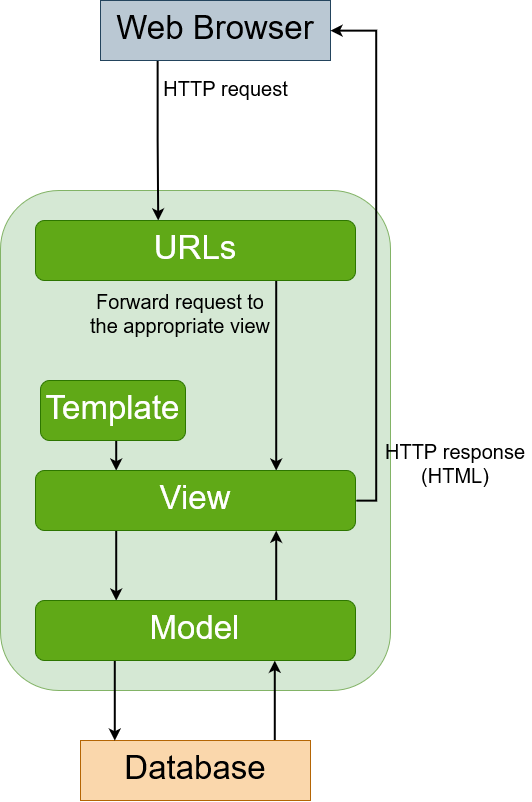
\includegraphics[scale=0.9]{images/Django_doc.png}
	\caption{Schema di funzionamento generico di un applicativo web sviluppato con Django}
\end{figure}

URLs: While it is possible to process requests from every single URL via a single function, it is much more maintainable to write 
a separate view function to handle each resource. A URL mapper is used to redirect HTTP requests to the appropriate view based on 
the request URL. The URL mapper can also match particular patterns of strings or digits that appear in an URL, and pass these to a 
view function as data.
View: A view is a request handler function, which receives HTTP requests and returns HTTP responses. Views access the data needed to 
satisfy requests via models, and delegate the formatting of the response to templates.
Models: Models are Python objects that define the structure of an application's data, and provide mechanisms to manage (add, modify, 
delete) and query records in the database. 
Templates: A template is a text file defining the structure or layout of a file (such as an HTML page), with placeholders used to 
represent actual content. A view can dynamically create an HTML page using an HTML template, populating it with data from a model. 
A template can be used to define the structure of any type of file; it doesn't have to be HTML!
\cite{mdn-django-documentation} \cite{django-documentation}



\section{Docker}
Docker è una piattaforma software che permette di creare, testare e distribuire applicazioni con la massima rapidità. Docker raccoglie 
il software in unità standardizzate chiamate container che offrono tutto il necessario per la loro corretta esecuzione, incluse librerie, 
strumenti di sistema, codice e runtime. Con Docker, è possibile 
distribuire e ricalibrare le risorse per un'applicazione in qualsiasi ambiente, tenendo sempre sotto controllo il codice eseguito.

La tecnologia Docker utilizza il kernel di Linux e le sue funzionalità, come Cgroups e namespace, per isolare i processi in modo da poterli 
eseguire in maniera indipendente. Questa indipendenza è l'obiettivo dei container: la capacità di eseguire più processi e applicazioni in 
modo separato per sfruttare al meglio l'infrastruttura esistente pur conservando il livello di sicurezza che sarebbe garantito dalla 
presenza di sistemi separati.

\begin{figure}
	\centering
	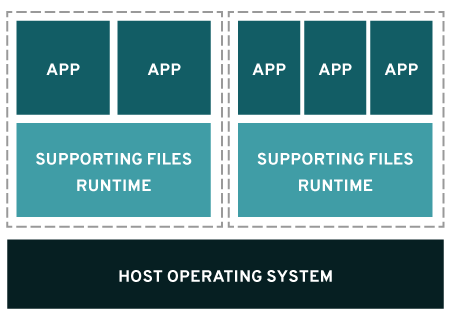
\includegraphics[scale=0.7]{images/Docker_Config_Container.png}
	\caption{Schematizzazione del contenuto di un Container di Docker}
	\label{fig:DCC}
\end{figure}

Gli strumenti per la creazione di container, come Docker, consentono il deployment a partire da un'immagine. Ciò semplifica la 
condivisione di un'applicazione o di un insieme di servizi, con tutte le loro dipendenze, nei vari ambienti.

Docker, considera i container come macchine virtuali modulari estremamente leggere, offrendo la flessibilità di creare, distribuire, 
copiare e spostare i container da un ambiente all'altro, ottimizzando così le app per il cloud.

\begin{figure}[H]
	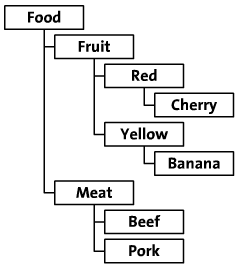
\includegraphics[scale=0.7]{images/Hierarchical_Data_ex.PNG}
	\caption{Esempio di una gestione di dati in modo gerarchico}
	\label{fig:Hde}
\end{figure}

I contenitori forniscono una modalità standard per impacchettare il codice della tua applicazione, le configurazioni e le dipendenze, 
in un oggetto singolo. I contenitori condividono un sistema operativo installato sul server e operano come processi con risorse isolate, 
assicurando velocità, affidabilità e distribuzioni coerenti, indipendentemente dall’ambiente.

\section{Strutture dati gerarchiche}
Le tabelle di un database relazione non sono gerarchiche (come nel XML), ma sono delle semplici liste piatte. I dati gerarchici sono 
constituiti da relazioni padre-figlio che non possono essere rappresentate in modo naturale nelle tabelle dei database relazionali.
In questo caso, i dati gerarchici sono una collezione di informazioni dove ogni item ha un solo padre e nessuno o più figli
(ad eccezione del nodo radice che non ha un nodo padre); questo genere di rappresentazione delle informazioni può essere trovato in 
diversi ambiti di applicazione di un database, incluse discussioni su forum e mailing list, grafici di organizzazione di un business, 
categorie per gestire contenuti e categorie di prodotti. \\

\newpage

Ci sono differenti modelli per poter gestire dati in modo gerarchico, i più importanti che sono stati presi in considerazione sono i 
seguenti:

\subsection{The adjacency list model}
Il primo approccio, e quello di più semplice implementazione, qui descritto è chiamato \textit{‘adjacency list model} o metodo ricorsivo;
è definito tale perchè per funzionare necessita solo di una funzione che itera per tutto l'albero.\\
In questo modello, ogni item (nodo dell'albero) nella tablla contiene un puntatore al suo item padre; invece il nodo radice avrà un puntatore a un valore
NULL per l'item padre.

\begin{figure}[ht!]
    \centering
	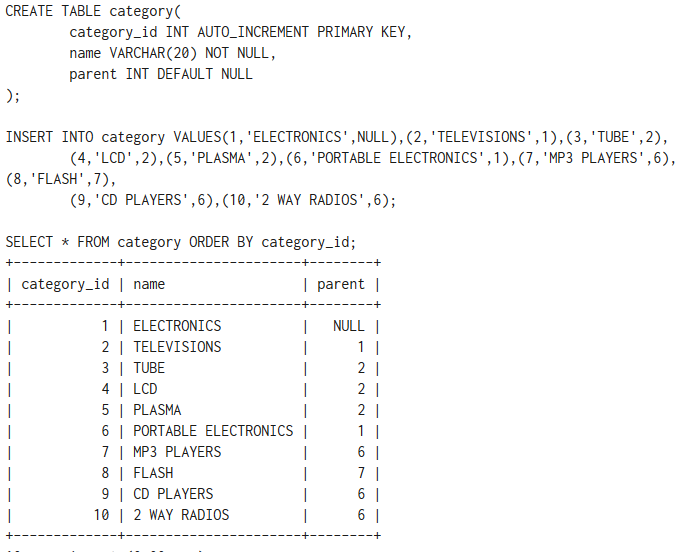
\includegraphics[scale=0.75]{images/Adjacency_list_model_table.PNG}
	\caption{Esempio di una tabella per gestire dati in modo gerarchico secondo l'adjacency list model }
\end{figure}
 
Il vantaggio di usare questo modello sta nella sua semplicità di costruzione sopratutto a livello di codice client-side, 
e di restituzione dei figli di un nodo. Mentre diventa problematico se si lavora in puro SQL e nella maggior parte dei linguaggi di 
programmazione, è lento e poco efficente, perchè è necessaria una query per ogni nodo dell'albero, e visto che ogni query impiega 
un certo periodo di tempo, questo rende la funzione molto lente quando si lavora con alberi di grandi dimensioni.
Inoltre molti linguaggi non sono ottimizzati per funzioni ricorsive. Per ogni nodo, la funzione inizia una nuova istanza di se stessa,
ogni istanza occupa una porzione di memoria e impiega un certo tempo per inizializzarsi, e più grande è l'albero e più questo 
processo sarà portato a termine in maggior tempo.

\subsection{The Nested set model}
Il secondo approccio che viene proposto è il \textit{Nested set model}, che permette di osservare la gerarchia in un modo diverso, non 
come nodi e linee, ma come container innestati. \\

\begin{figure}[ht!]
    \centering
	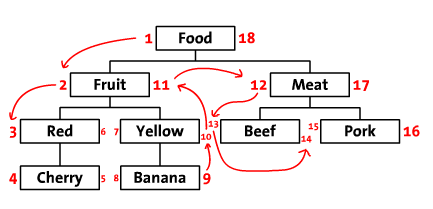
\includegraphics[scale=0.55]{images/Nested_Tree_Model_ex.PNG}
	\caption{Esempio di una gestione di dati in modo gerarchico secondo il Nested set model}
\end{figure}

La gerarchia dei dati viene rappresentata nella tabella attraverso l'uso degli attributi 'left' e 'right' per rappresentare l'annidamento
dei nodi (il nome delle colonne: left e right, hanno significati speciali in SQL; per questo motivo si identificano questi campi con i 
nomi 'lft' e 'rght'). 
Ogni nodo dell'albero viene visitato due volte, assegnando i valori in ordine di visita, e in entrambe le visite. Quindi vengono 
associati ad ogni nodo due numeri, memorizzato come due attributi. 
I valori di left e right sono determinati come segue: si inizia a numerare a partire dal lato più a sinistra di ogni nodo e si continua 
verso destra. Lavorando con un albero, si parte da sinistra e si continua verso destra, un livello alla volta, scendendo per ogni
nodo i suoi figli, assegnando i valori al campo left, prima di assegnare un valore al campo right, e successivamente si continua verso 
destra. Questo approccio è chiamato Modified preorder tree traversal algorithm.

A prima vista questo approccio può sembrare più complicato da comprendere rispetto all'adjacency list model, ma quest'utlimo metodo è
molto più veloce quando si vuole recuperare i nodi, visto che basta una query, mentre più lento per operazioni di aggiornamento e 
cancellazione dei nodi; in quest ultimo il grado di complicatezza dell'operazione è determinato dal nodo che si vuole cancellare, a 
partire dal caso più semplice, il nodo foglia (nodo senza figli) fino al caso più complicato, quando si vuole cancellare il nodo radice. \\

\begin{figure}[ht!]
    \centering
	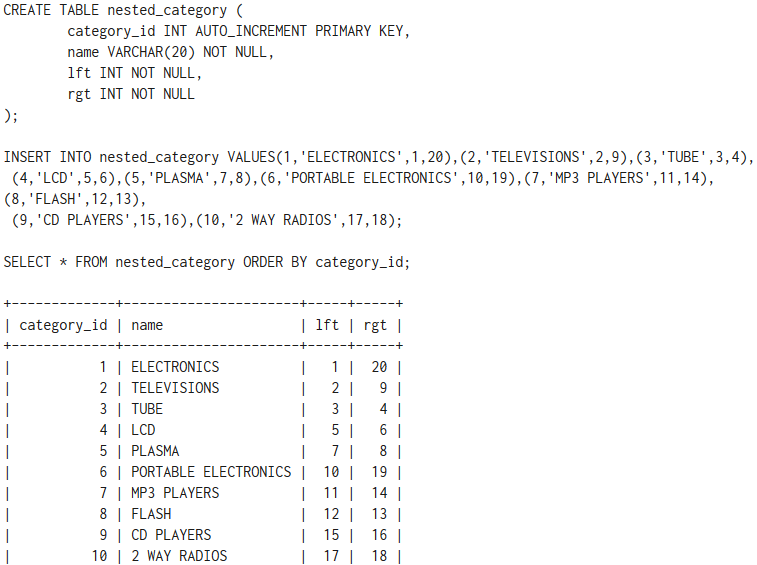
\includegraphics[scale=0.6]{images/Nested_Tree_Model_table.PNG}
	\caption{Esempio di una tabelle per la gestione di dati in modo gerarchico secondo il Nested set model}
\end{figure}

\newpage

\section{Sistemi di raccomandazione}
Un sistema di raccomandazione (\textit{Recommendation System}) è un sistema che raccomanda item ad utenti tra numerosi item esistenti 
in database. L'item è qualsiasi cosa che possa piacere agli utenti, come prodotti, libri e giornali. Si generano aspettative che 
l'item raccomandato possa essere tra quelli che sia di maggiore interesse; in altre parole, questi item particolari sono in accordo 
con i gusti degli utenti. 
\\
\\
Oggigiorno si possono trovare due trend di sistemi di raccomandazione: 
\begin{description}
	\item[Content-based filtering](CBF): un item viene raccomandato ad un utente se esso è simile agli altri item di interesse o piaciuti
	nel passato (la valutazione per questi item è alta o sono stati molto utilizzati). Da notare che ogni item ha delle informazioni che
	ne definiscono le caratteristiche e proprietà (spesso questo insieme di dati viene definito metadati), e sono fondamentali per il 
	processo di raccomandazione. 
	\item[Collaborative filtering](CF): un item viene raccomandato ad un utente se i suoi vicini (gli altri utenti simili) sono interessati
	a quell'item.   
\end{description}

Entrambi gli approcci (CBF e CF) hanno i loro punti di forza e di debolezza. Il primo algoritmo si focalizza sul contenuto degli item e
sugli interessi del singolo utente; raccomanda iteme differenti a utenti differenti. Ogni utente può ricevere raccomandazioni uniche; e 
questo è un vantaggio. Tuttavia CBF non si tende verso la comunità di utenti come il CF; per questo motivo si potrebbero tralasciare 
item di interesse ad un utente parchè nascosti all'interno della comunità, CBF non ha l'abilità di scoprire item in modo implicito; e 
questa è la sua più grande limitazione.
Se ci sono molti contenuti associati agli item (per esempio, un item ha molte proprietà) allora, il sistema CF consuma molte risorse e 
tempo per poter analizzare i dati, nel contempo a questo algoritmo non interessano queste informazioni. Una raccomandazione viene fatta
sulla base delle valutazioni degli utenti per gli item, o sugli usi che gli utenti fanno degli item; questo è il suo punto di forza 
perchè non si trova di fronte a dover analizzare item con un ricco contenuto. Allo stesso tempo è anche il suo punto debole, perchè può
portare a suggerimenti che potrebbero essere considerati poco adatti sulla base della poca relazione con i profili di alcuni utenti.

\begin{figure}[ht!]
	\centering
	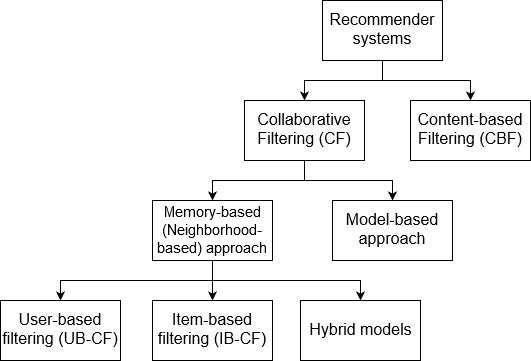
\includegraphics[scale=0.5]{images/recommender_systems.jpg}
	\caption{}
	\label{fig:RS}
\end{figure}


\cite{model-based-approach-for-collaborative-filtering}
Un sistema di raccomandazione filtra i dati usando differenti algoritmi e raccomanda gli item più rilevanti agli utenti,
attraverso un procedimento a 3 fasi:

\begin{description}
	\item[raccolta di dati]: questa è il primo step e anche quello più importante per poter costruire un sistema di 
	raccomandazione che produca risultanti rilevanti e consistenti. I dati possono essere raccolti in due modi: esplicitamente,
	cioè attraverso i dati che vengono prodotti direttamente dagli utenti, ad esempio le valutazioni di un prodotto; mentre 
	attarverso l'approccio implicito, vengono raccolti dati che non sono prodotti in modo intenzionale dall'utente ma raccolti
	dai costanti flussi di dati come la cronologia di ricerca, i click effettuati, lo storico degli ordini, etc.
	\item[memorizzazione di dati]: la quantità di dati definisce quanto efficace un modello di raccomandazione possa di
	diventare. Ad esempio, in un sistema di raccomanzione per film, maggiori sono le valutazioni fornite dagli utenti, e 
	migliore sarà il sistema di raccomandazione per gli altri utenti. Il tipo di dati che si vuole raccogliere determina
	anche il supporto di memorizzazione più adatto.   
	\item[Filtraggio dei dati]: dopo la fase di raccolta e memorizzazione dei dati, essi vanno filtrati per poter estrarre
	le informazioni rilevanti per poter effettuare le raccomandazioni finali, e sono già disponibili diversi algoritmi che
	semplificano quest ultima fase. 
\end{description}

I sistemi di raccomandazione possono essere suddivisi nelle seguenti categorie, ma speso si preferisco degli approcci imbridi cioè delle
combinazioni di sistemi di raccomandazione basati sul contenuto (\textit{Content-based filtering}) e 
quelli collaborativi (\textit{Collaborative filtering}) in modo da essere più efficaci sfruttando i pregi di entrambi gli approcci.


\subsection{Content-based filtering}
Un Content-based filtering è un sistema di raccomandazione in cui vengono suggeriti item simili a un particolare item (oggetti 
o prodotti). 

Questo approccio sfrutta i metadati dell'item, che possono essere il genere, una descrizione, uno o più autori, la categoria di 
appartenenza etc. per fare queste raccomandazioni; l'idea base che sta dietro questi raccomandatori, è che se ad un utente piace 
o interessa un particolare item allora gli piaceranno anche altri item simili.

Questo algoritmo suggerisce prodotti che piacevano all'utente nel passato ed è limitato a item dello stesso tipo. Un 
content-based recommender fa riferimento a quegli approcci, che provvedono raccomandazioni comparano la rappresentazione del
contenuto che descrive un item e la rappresentazione del contenuto dell'item interessato dall'utente. 

Questi metodi sono usati quando si sanno a priori delle informazioni sugli item che si vuole suggerire, ma non sugli utenti.
In questo sistema, delle keyword (parole chiave) sono utilizzate per caratterizzare gli item e un profilo dell'utente è 
costruito per indicare quali item gli piacciono. In altre parole, questi algoritmi cercano di raccomandare item che 
all'utente sono piaciuti o ha usato nel passato e sta esaminando nel presente. La costruzione del profilo dell'utente,
spesso temporaneo, non viene basata su un modulo di registrazione che l'utente stesso deve compilare, ma su informazioni
lasciate indirettamente dall'utente. Più precisamente, tra vari item candidati da raccomandare all'utente si passa per un 
processo di confronto con gli item piaciuti dall'utente e gli item migliori vengono suggeriti.


\subsection{Collaborative filtering}
I filtri collaborativi (\textit{Collaborative filtering}) lavorano costruendo un database di preferenze di utenti su item (o prodotti),
sfruttano tecniche di analisi dei dati al problema di aiutare gli utenti a trovare gli item che gli potrebbero piacere producendo una 
lista dei top-N item da raccomandare per un dato utente.
Un nuovo utente subisce un processo di matching all'interno del database per scoprire quali sono i possibili vicini (\textit{neighbors}),
che corrispondo agli altri utenti aventi storicamente simili preferenze al nuovo utente. Agli item maggiormente preferiti dai vicini sono
raccomandati al nuovo utente, visto che potrebbero essere di suo interesse. 

Questi sistemi tentano di predirre la valutazione o la preferenza che un utente darebbe a un item basandosi su preferenze date da altri 
utenti, queste preferenze possono essere ottenute o in modo esplicito dagli utenti o tramite qualche misurazione implicita. 
I filtri collaborativi non richiedono l'uso di metadati associati agli item come nella loro controparte, i filtri content-based. A un 
utente vengono raccomandati item basandosi su valutazioni passate collezionate da altri utenti.

Tuttavia, restano ancora oggi alcune sfide significative a cui sono sottoposti i sistemi di raccomandazione basati su 
filtraggio collaborativo.
Il primo obbiettivo è quello di migliorare la scalabilità degli algoritmi di filtri collaborativi; questi algoritmi sono in grado di cercare
anche diecimila di potenziali vicini (utenti simili) in tempo reale, ma la richiesta dei sistemi moderni è di cercare dieci milioni di 
potenziali vicini. Algoritmi esistenti hanno problemi di performance con i singoli utenti quando essi hanno molte informazioni.
Il secondo obbiettivo è quello di migliorare la qualità dei sistemi di raccomandazione per gli utenti. Gli utenti vogliono
raccomandazioni di cui possono fidarsi e che possono aiutarli a trovare item che potrebbero essere di loro gusto.
Per certi versi questi due obbiettivi sono in conflitto tra di loro e per ottenere dei risultati validi e di una certa importanza è 
necessario trattarli in contemporanea perchè aumentare solamente la scalabilità diminuirebbe la sua qualità e viceversa. 
\cite{item-based-collaborative-filtering} 

Il principale modello di filtro collaborativo studiato in questo elaborato è il metodo definito come \textit{Memory-based} e il 
vantaggio di utilizzare queste tecniche sta nel fatto di essere semplici da implementare e i risultati ottenuti sono altrettanto 
semplici da spiegare; mentre ci possono essere anche filtri collaborativi che sfruttano metodi \textit{Model-based} che si basano sulla 
fattorizzazione di matrici e sono molto più funzionali per gestire il problema della sparsità dei dati. Questi ultimi sono sviluppati
usando algoritmi di data mining e machine learning per predirre le valutazioni di utenti su item senza valutazioni, inoltre sono spesso 
associati a tecniche come la dimensionality reduction per migliorare la precisione.



\subsection{Challenges and limitations} \hfill \break
Cosa succederebbe se un nuovo utente o un nuovo item è aggiunto al dataset? Questa situazione è chiamata \textit{Cold Start}. Ci possono
essere due tipi di Cold Start:
\begin{description}
	\item[Visitor Cold Start]:
	\item[Product Cold Start]: 
\end{description}

Cold start problem
What will happen if a new user or a new item is added in the dataset? It is called a Cold Start. There can be two types of cold start:
	Visitor Cold Start: means that a new user is introduced in the dataset. Since there is no history of that user, the system does not 
know the preferences of that user. It becomes harder to recommend products to that user. So, how can we solve this problem? One basic
approach could be to apply a popularity based strategy, i.e. recommend the most popular products. These can be determined by what has
been popular recently overall or regionally. Once we know the preferences of the user, recommending products will be easier.
	Product Cold Start: means that a new product is launched in the market or added to the system. User action is most important to
determine the value of any product. More the interaction a product receives, the easier it is for our model to recommend that product
to the right user. We can make use of Content based filtering to solve this problem. The system first uses the content of the new 
product for recommendations and then eventually the user actions on that product.


  Cons
	Scalability: The more K neighbors we consider (under a certain threshold), the better my classification should be. 
  Nevertheless, the more users there are in the system, the greater the cost of finding the nearest K neighbors will be.
	Cold-start: New users will have no to little information about them to be compared with other users.
	New item: Just like the last point, new items will lack of ratings to create a solid ranking (More of this on ‘How to sort 
  and rank items’).

SPARSITY

Stated simply, most users do not rate most items and, hence, the user ratings matrix is typically very sparse. is is a problem for 
collaborative +ltering systems, since it decreases the probability of +nding a set of users with similar ratings. This problem often 
occurs when a system has a very high item-to-user ratio, or the system is in the initial stages of use. This issue can be mitigated by 
using additional domain information or making assumptions about the data generation process that allows for high-quality imputation.

